%\documentclass[11pt]{article}
%
%%\usepackage[margin=1.01in]{geometry}
%%\usepackage{mathpazo}
%\usepackage[utf8]{inputenc}
%\usepackage{NSFProposal}
%
%%\addtolength{\oddsidemargin}{-0.6in}
%%\addtolength{\evensidemargin}{-0.75in}
%%\addtolength{\textwidth}{1.2in}
%%\addtolength{\topmargin}{-0.75in}
%%\addtolength{\textheight}{1.4in}
%%
%%\usepackage[margin=1.02in]{geometry}
%%\def\baselinestretch{1}
%%\special{papersize=8.5in,11in}
%
%%\usepackage[left=1.1in, right=1.1in]{geometry}
%
%%
%\usepackage{url}
%\usepackage{amsfonts,amsmath,amssymb,amsbsy}
%\usepackage{latexsym}
%
%\usepackage{bm}
%\usepackage{comment}
%%\usepackage{upgreek}
%\usepackage{graphics,graphicx}
%\usepackage{psfrag}
%\usepackage{epsfig}
%\usepackage{wrapfig}
%\usepackage{mathrsfs}
%
%\usepackage{pgfgantt}
%\usepackage{subfigure}
%
%\usepackage[square,numbers,comma,sort&compress]{natbib}
%%\usepackage{hyperref}
%
%\usepackage{commath}
%\usepackage{array}
%%\newcommand{\todo}[1]{%
%%  {\bfseries\color{red} XXX TODO: #1}
%%}
%\usepackage[font=small,labelfont=bf,labelsep=period]{caption}
%%\usepackage[margin=30pt,font=small,labelfont=bf,
%%  labelsep=period,skip=10pt]{caption}
%
%\usepackage{todonotes}
%\usepackage{pgfplots,tikz,color,soul,array,enumitem}
%
%
%\newcounter{midequation}
%
%\newtheorem{definition}{Definition}
%\newtheorem{lemma}{Lemma}
%\newtheorem{example}{Example}
%\newtheorem{theorem}{Theorem}
%\newtheorem{proposition}{Proposition}
%\newtheorem{remark}{Remark}
%
%
%
%\newcommand{\diff}{\mathrm{d}}
%\newcommand{\intd}{\,\mathrm{d}}
%\newcommand{\kBT}{$\mathrm{k}_{\mathrm{B}}\mathrm{T}$}
%\newcommand{\KB}{k_{\mathrm{B}}}
%\newcommand{\KG}{k_{\mathrm{G}}}
%\newcommand{\KT}{k_{\mathrm{T}}}
%\newcommand{\KTH}{k_{\theta}}
%\newcommand{\KA}{k_{\mathrm{A}}}
%\newcommand{\eg}{{\it e.g.~}}
%\newcommand{\ie}{{\it i.e.~}}
%\DeclareMathOperator{\Div}{div}
%\DeclareMathOperator{\Curl}{curl}
%
%% Bryan's Marcros
%\renewcommand{\aa}{\mathbf{a}}
%\newcommand{\bd}{\partial}
%\newcommand{\dd}{\mathbf{d}}
%\newcommand{\DD}{\mathcal{D}}
%\newcommand{\eeta}{\boldsymbol{\eta}}
%\newcommand{\FF}{\mathbf{F}}
%\renewcommand{\gg}{\mathbf{g}}
%\newcommand{\GG}{\mathbf{G}}
%\newcommand{\JJ}{\mathbf{J}}
%\newcommand{\nn}{\mathbf{n}}
%\newcommand{\NN}{\mathbf{N}}
%\newcommand{\nnu}{\boldsymbol{\nu}}
%\newcommand{\ttau}{\boldsymbol{\tau}}
%\newcommand{\ssigma}{\boldsymbol{\sigma}}
%\newcommand{\rr}{\mathbf{r}}
%\newcommand{\RR}{\mathbb{R}}
%\renewcommand{\SS}{\mathbf{S}}
%\newcommand{\TT}{\mathbf{T}}
%\newcommand{\xx}{\mathbf{x}}
%\newcommand{\XX}{\mathbf{X}}
%\newcommand{\uu}{\mathbf{u}}
%\newcommand{\vv}{\mathbf{v}}
%\newcommand{\yy}{\mathbf{y}}
%\newcommand{\pderiv}[2]{\frac{\partial #1}{\partial #2}}
%\newcommand{\jump}[1]{[\![ #1 ]\!]}
%
%\begin{document}
%
%
%\newpage
%\pagenumbering{arabic}
%%\documentclass[10pt]{article}
\usepackage[utf8]{inputenc}
\usepackage{fullpage}
\pagestyle{empty}
\linespread{1.05}
\begin{document}
\section*{Summary}


\subsection*{Overview}
\vspace{-0.1in}
This proposal aims to advance mathematical modeling, analysis, and
numerical simulations of collective dynamics and self-assembly arising
from attractive interactions between dipolar/nematic particles in a
suspension. Physicists model such a self-assembly using particles
possessing a biphasic material label on either half, with one more
hydrophobic than the other. Hydrophobic surfaces experience a
non-additive long-range attraction called the hydrophobic force. This
force is a major source of nonspecific interactions in biology and soft
matter. Despite its ubiquity, theoretical developments explaining its
basic underlying principles have come relatively late. Motivated by its
broad applicability, the PIs recently developed a novel and intuitive
mathematical model, called the hydrophobic attraction potential model,
based on the linear response of water to surface perturbations. This
model was used to show, for the first time, self-assembly of such
bipolar particles into vesicle-like structures using moving domain
elliptic partial differential equations (PDEs).

%This proposal aims to advance mathematical modeling and analysis of
%collective dynamics of amphiphilic self-assembly. Amphiphilic particles
%such as lipid molecules possess both hydrophobic and hydrophilic
%surfaces and self-assemble into meso/macroscopic structures such as
%micelles and bilayers of lipids. Experimentalists model self-assembly
%using Janus particles—spherical particles possessing a biphasic material
%label on either hemisphere. Janus particles have been widely used in
%soft matter physics as a model amphiphilic colloid and can be designed
%for catalytic activity or stimuli-responsive smart materials.

%Hydrophobic surfaces experience a nonadditive long-range attraction
%called the hydrophobic force. This force is a major source of
%nonspecific interactions in biology and soft matter. Despite its
%ubiquity, theoretical developments explaining its basic underlying
%principles have come relatively late. Motivated by its broad
%applicability, the PIs recently developed a novel and intuitive
%mathematical model, called the hydrophobic attraction potential model,
%based on the linear response of water to surface perturbations. This
%model was used to show, for the first time, self-assembly of Janus
%particles into vesicle-like structures using a partial differential
%equation-based particle interaction.

The PIs propose to analyze the elliptic PDEs, develop fast and accurate
numerical algorithms, and apply their hydrophobic attraction potential
model to more general self-organization dynamics. They aim to generalize
the linear-response model to a wider class of hydrophobic interactions,
and numerically implement these interactions using integral equation
formulations. Finally, they will develop a coarse-grained model based on
the kinetic theory to investigate the rheological properties of the
assembly of particles with tunable hydrophobicity. The unifying aspects
of the project will establish a platform for efficiently simulating
the collective dynamics of large numbers of particles, and focus on
rigorous, mathematical analysis of the underlying model equations in
complex geometries. The project supports undergraduate and graduate
student collaborators.

\subsection*{Intellectual Merit}
\vspace{-0.1in}
This collaborative project focuses on modeling, simulation, and analysis
of self-assembly and collective dynamics of granules. The main
ingredient is a nonlocal interaction through the solution of an moving
domain elliptic PDE that encompasses long-range amphiphilic and
short-range steric interactions. The PIs have validated this
coarse-grained model against well-known vesicle hydrodynamics. The
technical research tasks include quantifying collective properties of
amphiphilic ensembles, improving on mathematical models, efficient,
high-order numerical algorithms for large-scale two- and
three-dimensional simulations with confinement, and developing a kinetic
theory for the collective dynamics.

%The purpose of this research is to reach interesting physical phenomena
%with less computational cost than molecular dynamics, and account for
%more general features that continuum theory misses. The main ingredient
%is defining a nonlocal interaction through the solution of an elliptic
%boundary value problem that has the phenomenological characteristics of
%long-range hydrophobic attraction. This minimal model, while intuitive,
%is quite a general description of amphiphiles in solvent and gives rise
%to rich phenomena from Janus particle aggregates to correctly predicting
%elastic properties of bilayer. The technical research tasks include
%quantifying collective properties of amphiphilic ensembles, improving on
%mathematical models, efficient, high-order numerical algorithms for
%large-scale simulations, and incorporating external fields through
%electric charge.

\subsection*{Broader Impacts}
\vspace{-0.1in}
This project aims to advance the mathematical modeling of collective
dynamics of amphiphilic granules. The framework uses a new PDE-based
formulation that accounts for important and complex systems in soft
matter. These complex systems include optimal shape design in
metamaterials and fusion and fission of amphiphilic bilayer membranes.
The simulations will be performed with computational tools designed to
solve the governing PDEs both efficiently and with high-order accuracy.
The models describing granular systems could be transformative in
biomedicine and material science. The research draws from expertise in
scientific computing, physics of fluids, and mathematics. The
mathematical component incorporates leading variational techniques and
offers insight into fundamentals of self-organization and collective
dynamics. The project brings socially consequential research into the
classroom and offers undergraduates the opportunity to train alongside
faculty and graduate students. With its unique combination of
mathematical modeling, analysis, and scientific computing, the project
highlights the potential advancement of STEM from applied mathematics.


\end{document}


%\pagestyle{empty}

\section{Specific Aim 1: Membrane vesicles as self-organized granules}
\label{sec:specific_aim1}
\subsection{Prior work related to the proposal.}

\subsubsection{Vesicles}
\begin{wrapfigure}[12]{r}{0.3\textwidth}
  \vspace{-5pt}
\centerline{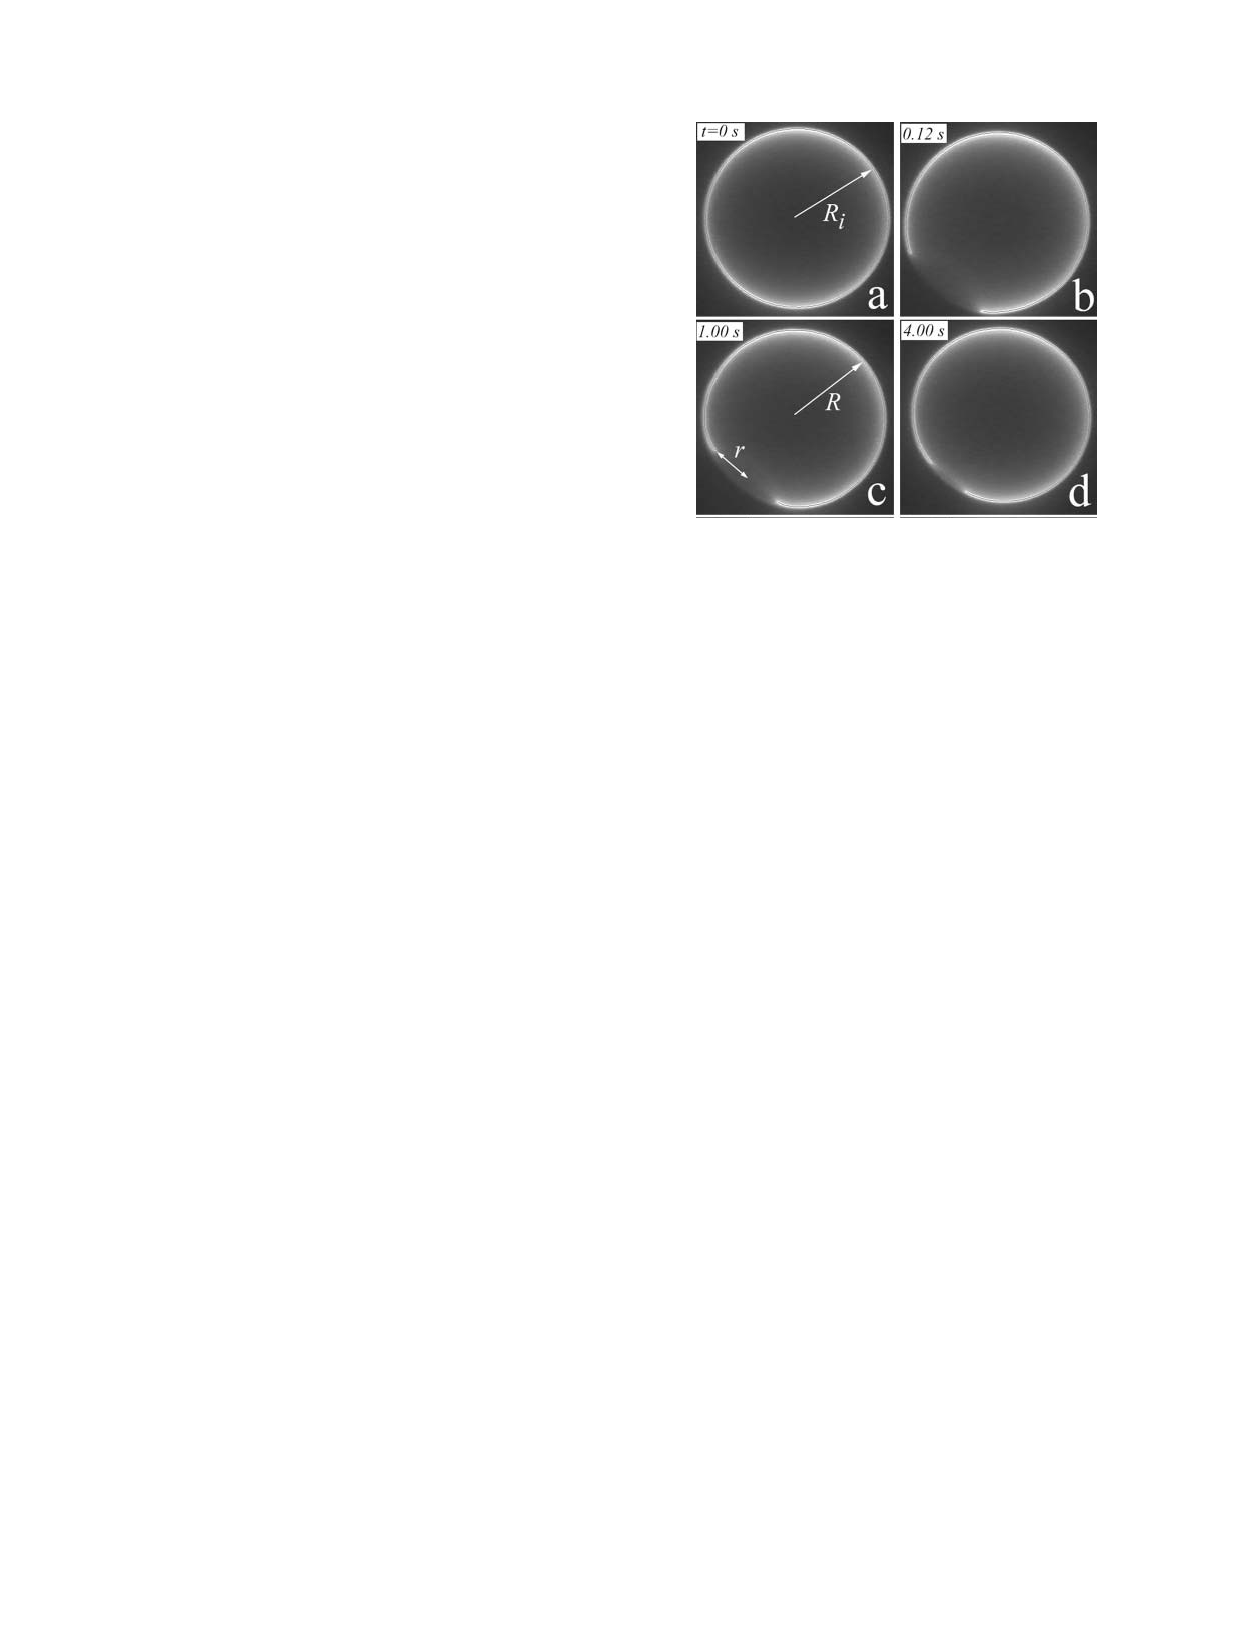
\includegraphics[width=0.3\textwidth]{figures/SA1Figures/LiposomePore.pdf}}
  \vspace{-5pt}
\caption{\label{fig:LiposomePore}Pore formation in a
stressed liposome~\cite{Kaetal03, BrdGSa00}.}
\end{wrapfigure}
PI Ryham has made fundamental contributions to interface modeling in
membrane biology.  His first works include
phase field formulations for the elastic bending energy \cite{0951-7715-18-3-016,Du05}
and 
topological indicators \cite{DuEuler} of vesicle membranes
and fluid-vesicle interactions \cite{QiangDu09}.
A decade ago, Ryham focused on the
problem of \emph{lipidic pore dynamics}.  
This problem came from 
experiments in the late 1990's 
showing that liposomes swollen by osmotic stress can form a single pore that
widens to allow the release of fluid (see Figure \ref{fig:LiposomePore}). 
Once pressure is released,
the widened pore closes according to a linear
followed by a square root law \cite{BrdGSa00}.  Researchers have
used the rates of pore closure to infer properties of the lipid membrane \cite{PoDi10}. 


In \cite{BrdGSa00}, 
physicists Olivier Sandre and Fran\c{c}oise Brochard-Wyart
and Nobel laureate Pierre-Gilles de Gennes
(PGG) formulated
rate equations for lipid pore dynamics.  These equations couple
the liposome stretching tension, pore edge tension, and membrane
dissipation.  A coefficient $C$ accounting for dissipation due to water
movement, however, was left unspecified because the Stokes flow
problem for the fluid surrounding a spherical cap with a moving hole
was unknown at the time \cite{Ra73}.  PI Ryham approached this problem using
a two-phase field method model \cite{RyCoEi12} and in a much-cited work
(coauthored with an undergraduate math major) by
fitting a dissipation coefficient $C \approx 8$ to data.
data \cite{RYHAM20112929}.  Finally, in the sole-author 
JFM paper \cite{Ryham2017OnTV},
Ryham solved the Stokes flow problem for
a moving pore completely yielding a value 
$C = \frac{4}{\pi}\csc \alpha\cot^2\frac{\alpha}{2}(\alpha - \sin \alpha + \alpha^2 \tan \frac{\alpha}{2})
~\sim 2\pi + 5(\alpha - \pi)$ in the pore angle $\alpha$.
Olivier Sandre wrote about the publication of the PI’s JFM paper:

\begin{quotation}“Maybe you can tell them this story: In my thesis
paper with Brochard \& PGG we got a factor of 8 wrong in determining
the viscosity of lipid membranes until a math teacher from the
Bronx corrected the model prefactor!”  Sandre, Olivier @Olive\_Free.
Twitter, January 3, 2018, https://twitter.com/Olive\_Free/status/948640705362169857
\end{quotation}

\begin{wrapfigure}[14]{l}{0.4\textwidth}
  \vspace{-5pt}
\centerline{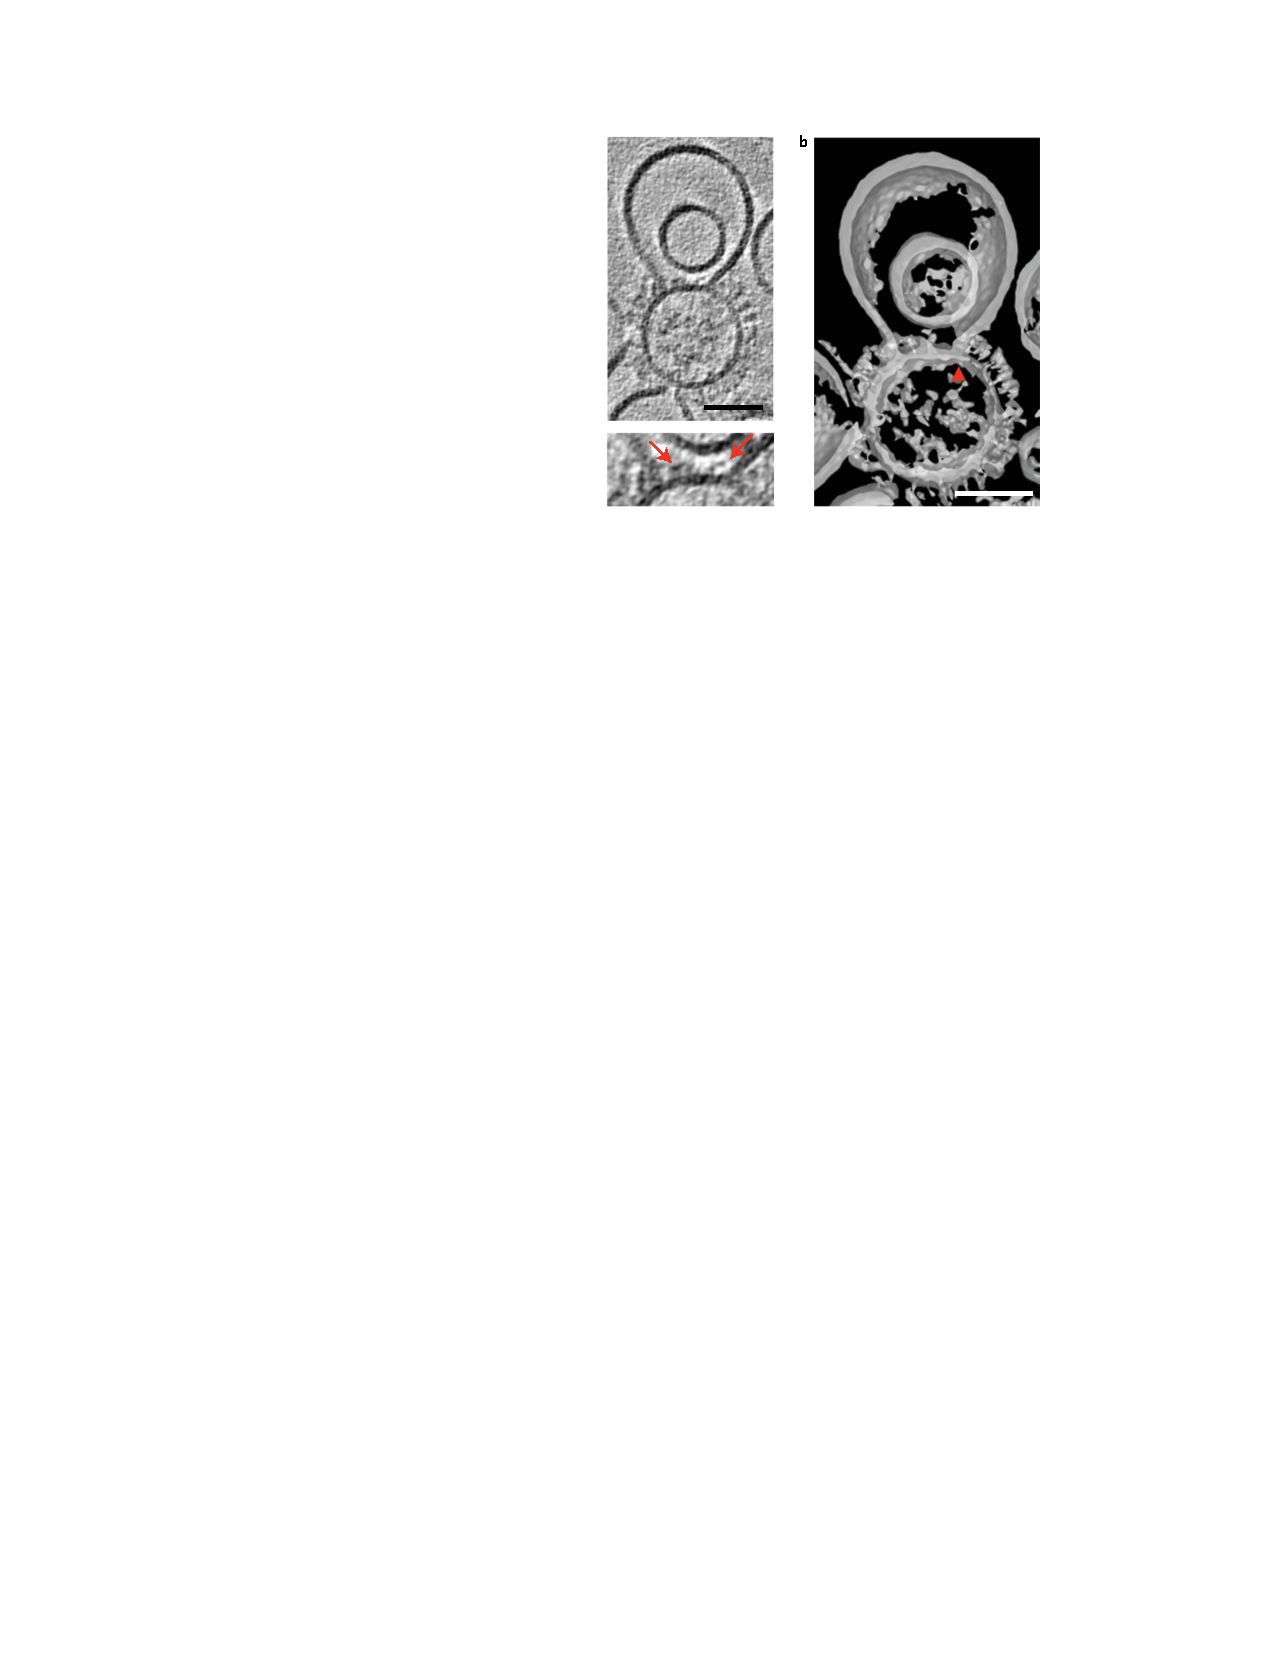
\includegraphics[width=0.4\textwidth]{figures/SA1Figures/FusionMicroscopy.pdf}}
  \vspace{-5pt}
\caption{\label{fig:FusionMicroscopy}
Fusion of an influenza virus-like particle with a liposome resolved
by electron tomography
~\cite{Chetal16}.}
\end{wrapfigure}

\noindent\textbf{Membrane Fusion.} Ryham has contributed
physically relevant, state-of-the-art methods in the
area of \emph{membrane fusion} (see Figure \ref{fig:FusionMicroscopy}).
Membranes fuse as a part of many biological
processes such as synaptic transmission, intracellular trafficking,
fertilization, and viral infection, and  a major challenge
to determine the forces needed to merge two lipid bilayers
~\cite{chernomordik2008mechanics, kozlov1982possible, Kuzmin19062001, markin2002membrane, qian2012novel}.  
Studying fusion is such a difficult problem because bilayers
consist of two monolayer surfaces coupled by a pair of surface vector fields
that model the elongated lipids. 


In his much noticed Biophysical Journal
and Nature papers~\cite{RyKlYaCo16,Chetal16}, Ryham and collaborators 
calculated, for the first time, a least energy path for membrane fusion.  
One mathematical innovation of this paper was to combine
the underlying surface-director model  with the simplified string method 
introduced by Weinan E, Weiqing Ren, and Eric Vanden-Eijnden
~\cite{doi:10.1063/1.2720838}
to calculate the saddle point separating two energy basins. 
The results~\cite{RyKlYaCo16} yielded energy barriers for stages of fusion
consistent with predictions from prominent MD and experimental groups
\cite{SmRiMu19,2017PNAS..114.1238F}.
The PI's papers ~\cite{RyWaCo13} and ~\cite{RyKlYaCo16} 
were also coauthored with undergraduate
mathematics majors.

\begin{wrapfigure}[10]{r}{0.4\textwidth}
  \vspace{-5pt}
\centerline{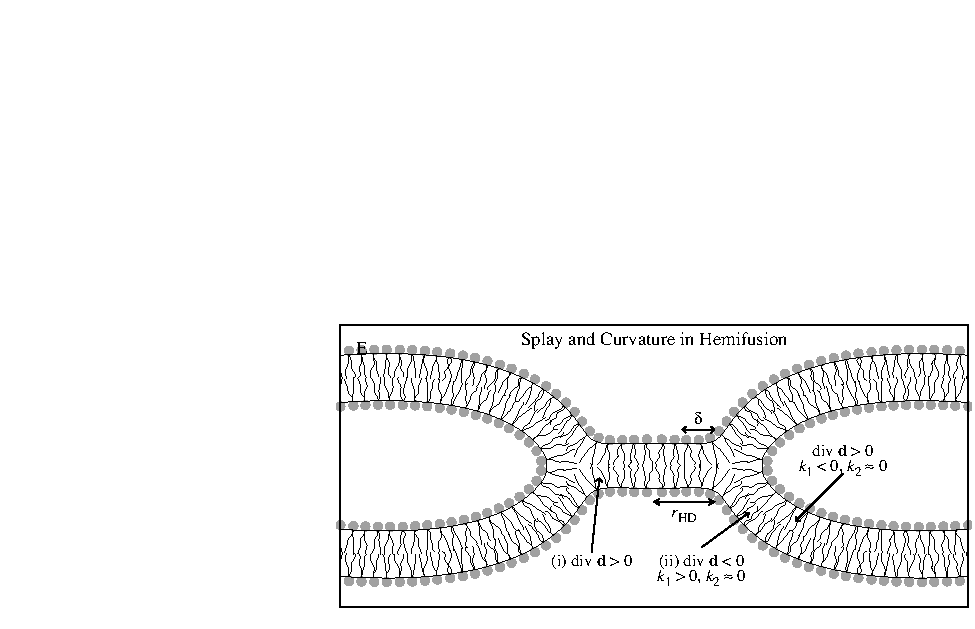
\includegraphics[width=0.4\textwidth]{figures/SA1Figures/Hemifusion.pdf}}
  \vspace{-5pt}
\caption{\label{fig:Hemifusion}
Axisymmetric hemifusion stage of two planar bilayers~\cite{RyKlYaCo16}.
Bilayer energy depends not only on surface curvature, but lipid orientations as well.}
\end{wrapfigure}
Phase field methods have been used to
study fusion in two dimensions~\cite{C9SM01983A} (MORE REFS), 
but these models do not resolve lipid orientations that play a crucial
role in processes like fusion.

\subsection{Vesicles as self-organized granules}
Interface problems coming from biology are a challenging
area of applied mathematics.  Broadly speaking, these problems
involve a fluid structure interaction where the modeler must
solve for the velocity in the aqueous phase, track the interface,
and couple the velocity boundary condition to the interface through
stress balance boundary conditions.  The aqueous phase can
be a low Reynolds number fluid, a porous medium, or viscoelastic fluid,
and the interfacial forces can come from surface tension, elasticity,
or electrostatics.
One typically enforces constant volume constraints through a no-slip
boundary condition for the velocity; if the interface is area incompressible
then one can additionally require that the velocity surface divergence
be zero.  Incorporating all these details can lead to models with substantial
complexity.

\subsubsection{Mathematical innovations.}
We developed the model \eqref{eqn:stokes}-\eqref{eqn:hydro_stress} 
as a robust and flexible approach
that cuts across many of the aforementioned challenging aspects to vesicle modeling.
\begin{enumerate}
\item The granules are not fixed to a stencil which
affords greater flexibility in terms of vesicle morphology 
and topological changes--sufficiently large forces will pull the granules apart 
as physically required,
\item An elliptic PDE \eqref{eqn:phase} provides the attraction that binds granules together,
opening the possibility for mathematical analysis, 
\item The model includes important details like lipid orientations and inter-monolayer
slip not present in diffusive interface models, and
\item With the help of boundary integral equations
and fast summation methods, the dynamics can be solved in 
near-linear complexity in $N_b$, which is equal to or better than 
that of related sharp interface methods. 
\end{enumerate}
The main insight that leads a collection of granules to form bilayers
is to define a so-called ``amphiphilic'' boundary condition for \eqref{}
It takes the form:
\begin{equation}
\label{eq:amphiphilic_BC}
h_i(\mathbf{x}) = \tfrac{1}{2}\left(\dd_i \cdot (\xx - \aa_i)/c_i + 1\right)
\end{equation}
where $\dd_i$ is the director, $\aa_i$ is the center, and $c_i$ the
``radius'' of the $i$th granule.  Inspired
by the amphiphilic structure of lipids, 
\eqref{eq:amphiphilic_BC} 
takes values close to $1$ on in the direction $\dd_i$,
representing a hydrophobic tail, and values close to $0$ 
in the direction $\dd_i$ representing the hydrophilic head.
%\begin{figure}
%Wrapped figure: a picture of a lipid and the granule geometry.
%\end{figure}

\begin{wrapfigure}[13]{r}{0.5\textwidth}
  \vspace{-5pt}
\centerline{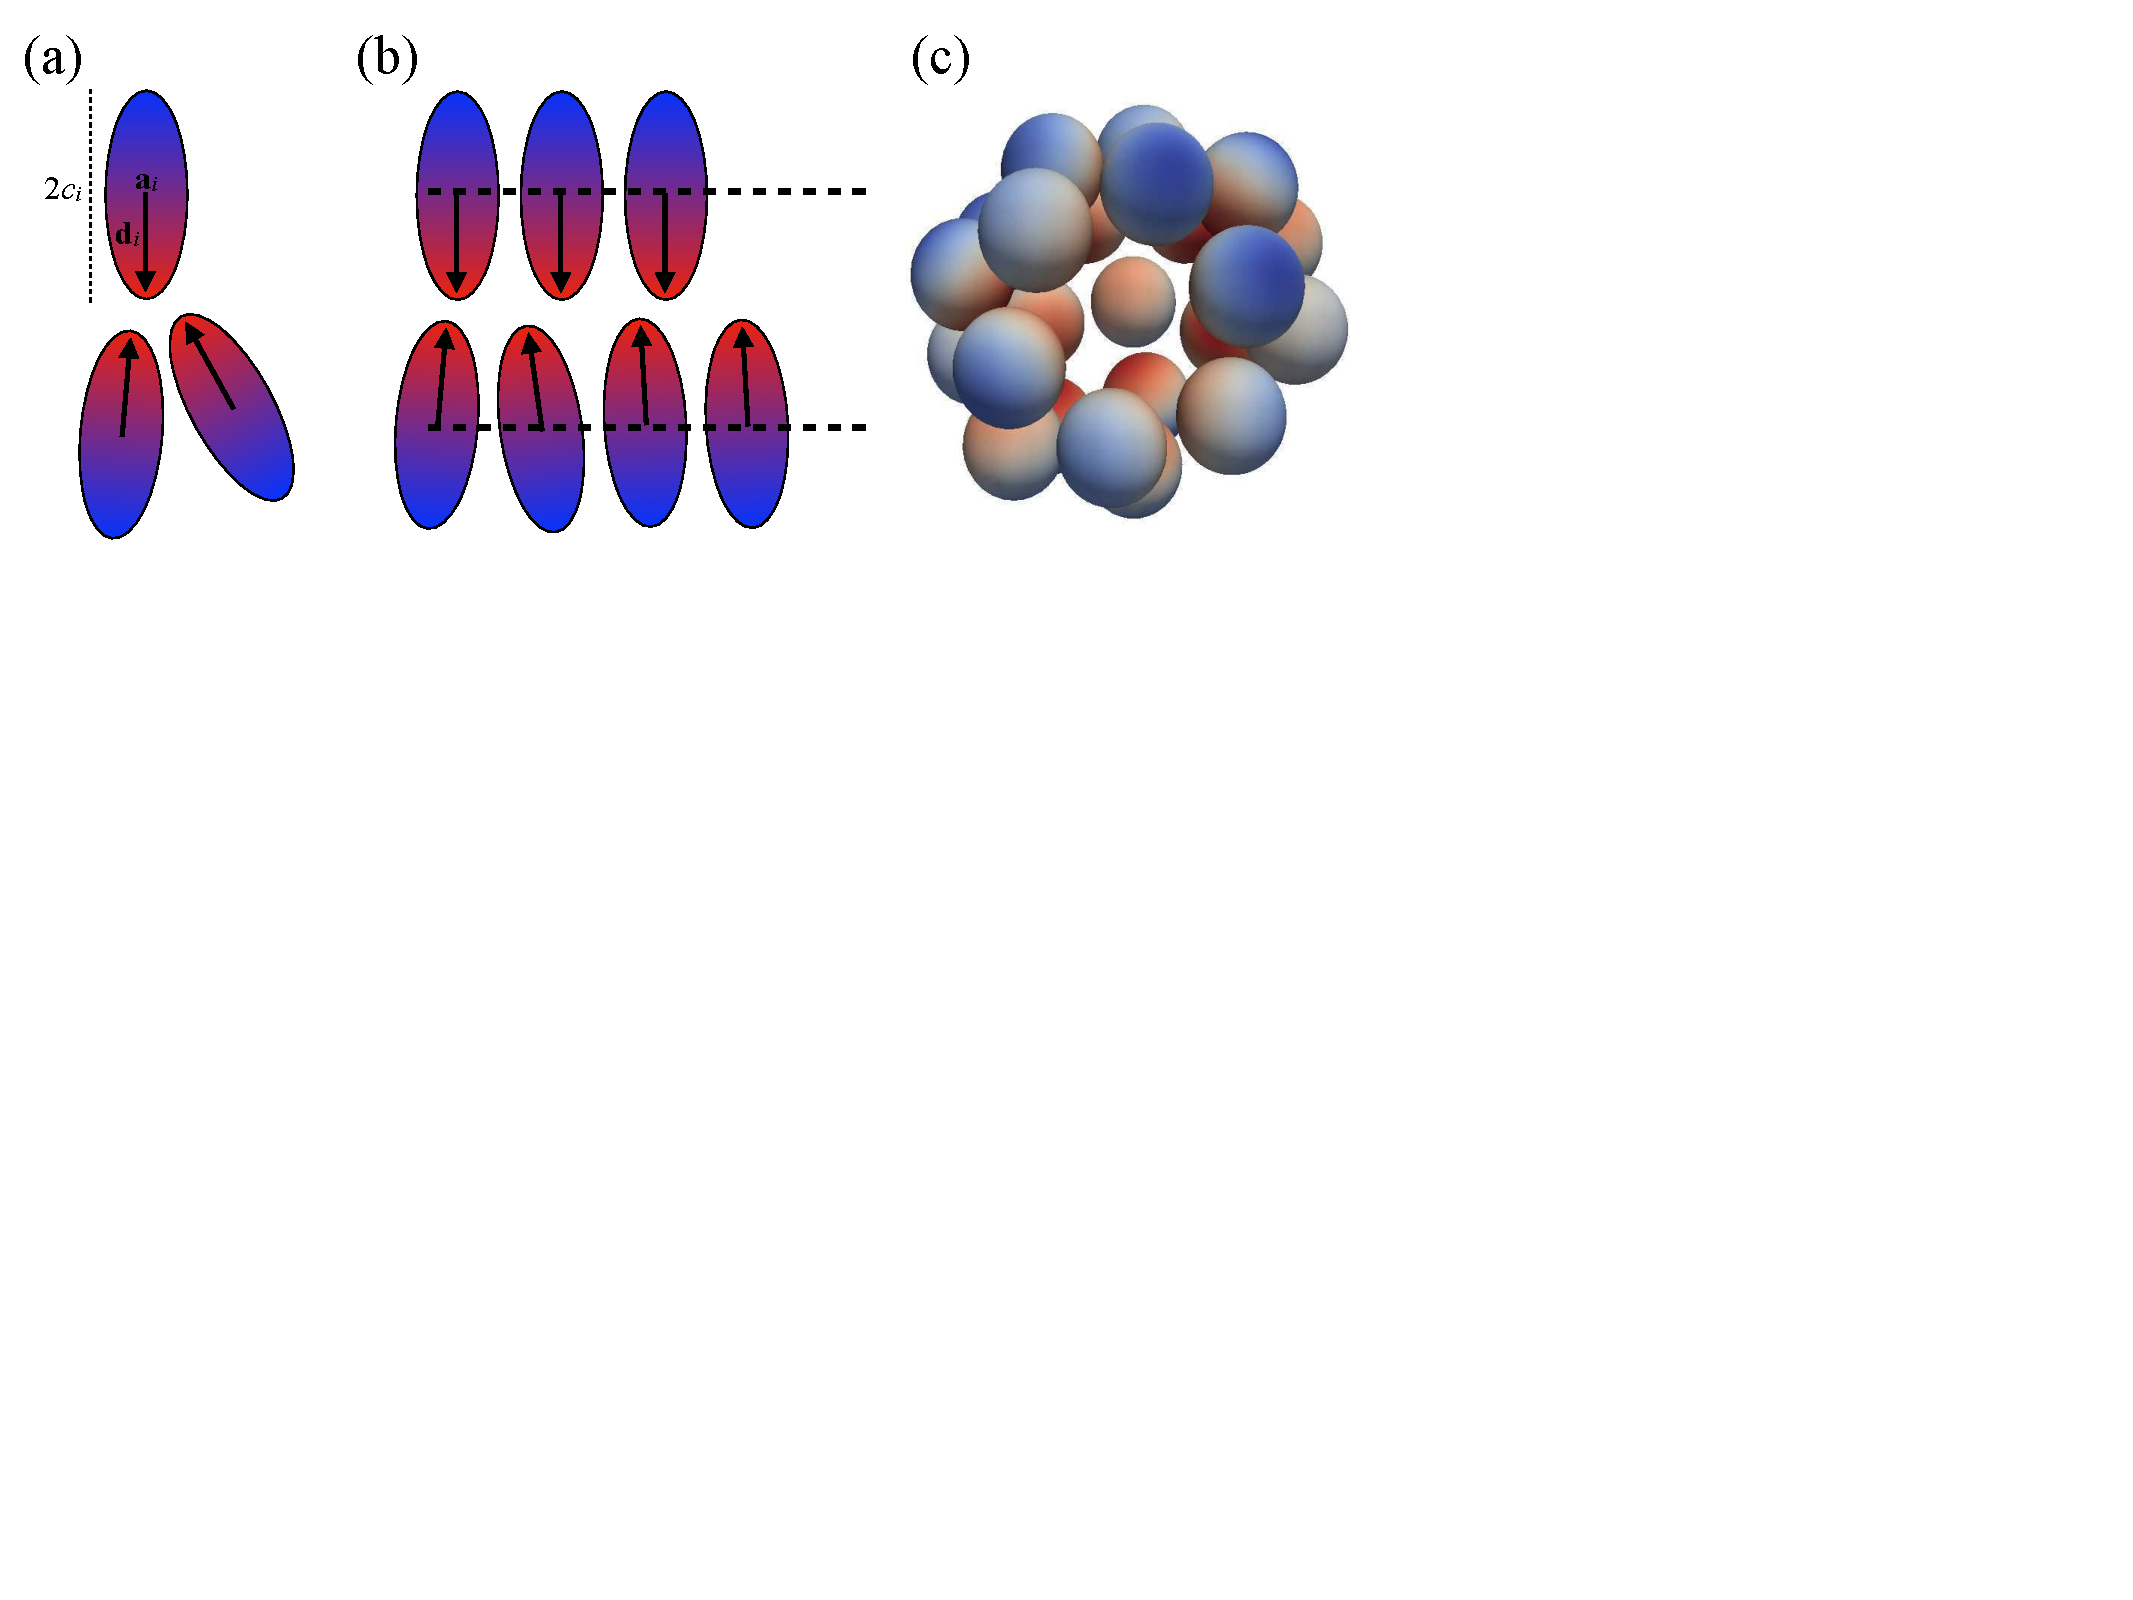
\includegraphics[width=0.5\textwidth]{figures/SA1Figures/AmphiphilicAssembly.pdf}}
  \vspace{-5pt}
\caption{\label{fig:amphiphilic_assembly}
Self-organization under amphiphilic boundary condition \eqref{eq:amphiphilic_BC}.
Granules first match hydrophobic tails (red) (a), then align length-wise (b). 
The behavior is the same in three dimensions 
as simulated by Kohl, Corona, and Veerapaneni
\cite{koh-cor-che-vee2021}.}
\end{wrapfigure}
The basic self-organization proceeds in two steps.
(a) Supensions of granules first minimize energy by matching hydrophobic
hydrophobic tails with one or more apposing granules
(Figure \ref{fig:amphiphilic_assembly}a, red regions.)
Once matched, there is still some residual energy in the
exposed sides.  In the minimimal configuration, pairs of
granules line up side by side, forming a bilayer,
and sequestering the hydrophobic
phase to the smallest possible region
(Figure \ref{fig:amphiphilic_assembly}b).
For numerical stability and physical realism,
we include a repulsion to prevent the granules from colliding.

\subsubsection{Do granule-based vesicle behave like continuum vesicles?}
A vesicle is a ring-shaped (or sphere-shaped in $\mathbb{R}^3$) 
and we analyze its energy as follows:
\begin{enumerate}
\item[Bending]
  The vesicle has bending energy because the directors are not
  parallel.  In the outer layer, the directors have negative
  splay $\nabla \cdot \dd < 0$ and in the inner layer
  the directors have positive splay $\nabla \cdot \dd > 0$.
  Due to minimality, the energy depends locally quadratically
  on the splay and has a bending modulus $k_B$.
  When $\dd$ is everywhere parallel to the unit normal $\NN,$ then
  \[
  \nabla \dd = -2H
  \]
  where $H$ is the mean curvature. 
\item[Stretch]
  If the vesicle is stretched, then the distance between
  neighboring granules is increased from rest.  The energy
  for this increase is Hookean and for small deformations
  equals
  \begin{equation}
    \label{eq:stretch}
    \tfrac{1}{2}k_A(L - L_0)^2/L_0
  \end{equation}
  where $k_A$ is a stretching modulus, $L$ and $L_0$ are stretched
  vesicle length and length at rest, respectively
  ($\tfrac{1}{2}k_A(A - A_0)^2/A_0$ in three dimensions).
  If the stretching is too great, the vesicle ruptures
  and the free eneds either rejoin, repairing the vesicle,
  of move apart forming a flat bilayer.
\item[Tilt]
  The directors in Figure \ref{} are normal to the vesicle surface.
  However, there are situations where the directors are not normal
  to the surface and this introduces the tilt angle $\theta$
  given by $\cos \theta = \dd \cdot \NN$.
  The energy for tilt is also Hooken and behaves like
  $k_{\theta}|\dd \times \NN|^2$ for the tilt modulus $k_{\theta}$.
\end{enumerate}

With regard to vesicle membranes and bilayers, two prominent 
classes of models researchers consider are the
Canham-Helfrich model and the more general Helfrich model.
In the Canham-Helfrich model, the membrane is assumed to have
negligible thickness and the lipids that form the membrane bilayer
are normal to the interface $\Sigma$.  The elastic energy takes the form
\begin{equation}
\label{eq:Canham-Helfrich}
  \int_{\Sigma} k_B(H - k_0)^2 + k_{\theta} \sigma\, dS 
\end{equation}
where $H$ is the mean curvature, $k_0$ is a spontaneous curvature,
$G$ is the Gaussian curvature, and $k_B$, $k_G$, $\sigma$, and $\gamma$ are
moduli for bending, saddle splay, surface tension, and line tension, respectively. 
If $\Sigma$ is a closed surface, then the integral
of Gaussian curvature is constant due to the Gauss-Bonnet Theorem.

This is our first step to showing the energy of the granule-based
vesicles have the same elastic energy as bilayers in the limit $N_b \to \infty$.
Once we have simulations for large systems sizes, we can provide
evidence that the two formulations are the same.
So and so has made simulations with thousands of granules in three-D
and this is now a technical/not theoretical limitation. 

\subsubsection{Do granule-based vesicles share hydrodynamic behavior of continuum vesicles?}

\begin{figure}R
  eview bend/stretch/tilt experiments
\end{figure}
\subsection{Vesicles in background flows}
\begin{itemize}
\item pull from JFM paper
\item we will consider background flows ...
\item results, rupture, critical shear rate
\item extensional flows
\item Taylor green flows; reorganization; do not know critical flow rate yet
\end{itemize}

\begin{remark}
  Mathematical problems: well-posedness of the system;
  Extensions to problems with transport;
  Calc-variational problem; place granules on fixed curve; study PDE system in
  SL -> 0; radius -> 0; Nb -> infty limit
\end{remark}
\begin{remark}
  In biophysics, tilt is defined by the tilt vector
  $\TT = \dd/\dd\cdot \NN - \NN$ so that the tilt energy density
  behaves like $\tan^2 \theta$ rather than $\sin^2 \theta$.
  These two energies densities are, however, asymptotically equal
  for small deformations.
Hamm and Kozlov [] and later Terzi and Deserno [], Pinigen et al. []
showed that the full Helfrich elastic energy of a \emph{monolayer} takes the form
\begin{equation}
\label{eq:Helfrich}
  \begin{aligned}
 &\int_{\Sigma}
  %\label{eq:Pinigan}
\tfrac{1}{2}k_{b}[(\nabla \cdot \mathbf{d} + k_{0})^{2} -  k^{2}_{0}]  
+ \tfrac{1}{2}k_{\theta}\mathbf{T}^{2} + \tfrac{1}{2}k_a[(\alpha - \alpha_0)^2 - \alpha_0^2] \\
&+ k_{c}\textbf{T} \cdot \nabla \nabla \cdot \mathbf{d}  + \tfrac{1}{2}k_{g}(\nabla \nabla \cdot \mathbf{d})^{2}
 + A\alpha \nabla \cdot \mathbf{d}
+ B \mathbf{T} \cdot \nabla \alpha \\
&- \tfrac{1}{2}k_c |\nabla \alpha|^2 + C \nabla \alpha \cdot \nabla \nabla \cdot \mathbf{d}\,dS
\end{aligned}
\end{equation}
where $\nabla$ and $\nabla \cdot$ are the surface gradient and surface divergence,
respectively, and $k_B$, $k_{\theta}$, $k_a$, $k_c$, $k_g$, $A$, $B$, $C$ are
appropriate elastic moduli.  An important and consequential distinction between
\eqref{eq:Canham-Helfrich} is the presence of the terms $\mathbf{T}$ and $\alpha$.
These are, respectively, the \emph{tilt} vector $\mathbf{T}$ measuring
the difference between the lipid director $\mathbf{d}$ and the surface normal
$\mathbf{N}$; the \emph{area per lipid} $\alpha$ area density at rest $\alpha_0$.
The two models \eqref{eq:Canham-Helfrich} and \eqref{eq:Helfrich} agree
when $\mathbf{T} = 0$ and $\alpha = \alpha_0$ everywhere.
\end{remark}



(Researchers Take from former background grant)

In biological processes like fusion and fission, however, the length scales of the
deformation (tens of nanometers) are comparable to membrane thickness (about 5 nm)
and so the detailed structure of bilayer cannot be ignored.
These models assign a surface $\Sigma$ to each of the two monolayers
of a bilayer, and a director field $\mathbf{n}:\Sigma \to \mathbb{R}^3$
for lipid orientation. Under very general continuum mechanical assumptions,

(Surface-director models).

The holy grail of biologically inspired fluid-interface models is
to have a formulation sufficient detailed and robust to make predictions
about biological processes.  Here, the Helfrich and Canham-Helfrich models
used throughout the field unfortunately fall short. For one,
realistic membranes are composed of a mixture of lipid species proteins.
Secondly, the membranes of living cells are constantly changing topology,
whether through fusion and fission with other membranes, or through
insertion or penetration by proteins and peptides.  Topological
changes are clumsy to incorporate into 
sharp interface formulations of the Helfrich and Canham-Helfrich energies
since computations rely on a parametrized surface of fixed topology.
Topological changes are permitted in phase field and level set formulations
of \eqref{eq:Canham-Helfrich}, but these methods smear out the 
details of lipid orientations, for example, that are important to the
process.  Recent work by [] and [] have incorporated lipid mixtures in \eqref{eq:Canham-Helfrich}
(although not \eqref{eq:Helfrich}), but these models have formidable complexity
due to the additional constraints and transport equations involved.

Nematic liquid crystals on surfaces is a related are of study.  These models,
which are closely related to \eqref{eq:Canham-Helfrich}, consider the energy
of a nematic liquid crystal (or Q-tensor ?) on a surface to study how the
surface geometry effects the director field and vice versa. Researchers
have formulated finite element methods for [][] and studied the existence
of minimizers []-[].  Liquid crystals are an extremely well-studied
are in mathematics [], where there are still a lot of open problems.

\begin{figure}
True bilayer; vesicle zero thickness; phase field; surface director
\end{figure}

We introduces \eqref{}-\eqref{} to overcome the challenges faced by
traditional Helfrich-type models of elastic membranes.

\noindent\textbf{Modeling vesicles} To make granular surfaces, we
form a collection of amphiphilic granules.  The granules have a
director $\mathbf{d} \in \mathbb{R}^n$ and the boundary condition
$g$ takes the form
\begin{equation}
g(\mathbf{x}) = \frac{1}{2}(\mathbf{d}\cdot(\mathbf{x}-\mathbf{a})/c + 1)
\end{equation}
where $c$ is granule radius.
This $g$ is smooth (real analytic even)
and takes values close to $1$ on the pole in the direction $\mathbf{d}$,
representing a hydrophobic face, and values close to $0$ on the pole
in the direction $-\mathbf{d}$ representing the hydrophilic face.
Then we define the well potential $f(\eta) = \tfrac{1}{2}\eta^2.$
This way, the hydrophilic side has the same phase as the bulk
($\eta = 0$, the minimum of $f$) and the hydrophobic side has
a higher potential energy phase.

Using \eqref{}-\eqref{}, suspensions of these granules self-organize
so that (i) apposing hydrophobic sides abut and (ii) granules align
side by side into sheets.  Vesicles are a stable configuration
of this process and the self-organization automatically expels or
absorbs the number of granules needed to minimize frustration between
the two leaflets.  But even for random initial configurations,
the granules form a collection of small vesicles and bilayer segments.
These disordered collections typically represent a local energy minimum 
because under a slight perturbation, the small vesicles and segments
further combine to form larger, stable vesicles.  

A natural questions concerns the well-posedness
\eqref{eq:RBT}--\eqref{eqn:stressbalance}
and its generalizations. A recent and strongly developing direction in
the area of nematics liquid crystals concerns the interaction of
Landau de Gennes functionals like \eqref{eq:energy_law} with colloids
\cite{doi:10.1098/rsta.2020.0432}.
In this spirit, a first step to understand the effect of the flow
in our model is to obtain some solid well-posedness results.

\begin{quotation}
  \textbf{Problem 1.} Consider a collection the closed,
  disjoint granules $U_i$ with smooth boundary,
with no-slip, rigid body motion boundary conditions.
Assume a either a single or double well potential
and a smooth phase field boundary condition.  
Study the well-posedness of the coupled system
\eqref{eq:RBT}--\eqref{eqn:stressbalance}
for short times.  For global in time solutions, determine
whether lubrication forces ensure positive distance
between granules.  Describe the behaviour in the limit
zero screening length limit.  
\end{quotation}

This problem is attractive because combines the diffusive interface
effects involving a free boundary in aqueous part of the region \cite{}
with interfacial effects coming from the long range inter-granual
attraction. Generalizations of Problem 1 include modifying the 
system to account for various time scales.
We may consider, for example, modifying \eqref{eqn:phase}
to include transport of the phase field by the background fluid;
\begin{equation*}
\phi_t + \uu \cdot \nabla = -\lambda \frac{\delta E}{\delta \phi} = \lambda(\epsilon^2 \Delta \phi - W'(\phi))
\end{equation*}
The modified systems enjoys the same energy law as \eqref{eq:energy_law} 
except that there will be an addtional dissipation term coming from the
Euler-Lagrange derivative $\frac{\delta E}{\delta \phi}$.

The second problem we consider concerns the approximation
of equilibrium elastic energy of curves and surfaces.
We have compared two-dimensional configurations of amphiphilic granules
to membrane configurations found in continuum mechanics.
The simulations results in~\cite{Fu2018_SIAM,FuQuRyYo22}
showed that the granular bilayers 
basically replicated the elastic energies for bending, tilt, and
stretching
but we do not yet have any analytical evidence to support this conclusion.
To understand the approximation mathematically, we take the following:
\begin{quotation}
  \textbf{Problem 2.} Place a collection of
  amphiphilic granules
with equally spaced centers along a curve $\mathcal{C}$.
For simplicity, assume that the directors are normal to the curve
and that the granules are all disks with radius proportional to $\epsilon$. 
Study the sharp interface limit of the energy $E$ 
relative to that of an array of granules placed along a flat curve. 
In this limit, the number of granules $N_b$ goes to infinity
to ensure equal spacing.
Study how the bending the bending $k_B$ and stretching $k_A$ coefficients
depend on the granual size relative to their spacing.
Generalize the problem to account for aspect ratio of elliptical granules
and nonzero tilt. 
\end{quotation}
Given the relatively complicated geometry consising
of a plane with a number of disjoint disks removed, 
we can start by approaching the problem in a simplified
setting such as when the reference curve is a circle.
There is a large body work in this direction for nematics
studying either the case of a single coloidal particle and
the qualitative structure of defects around it
\cite{Alama2015MinimizersOT, Alama2021SaturnRD, PhysRevE.96.042702}
many particles and the homogenization effects
\cite{Canevari2019DesignOE,doi:10.1137/18M1163919,doi:10.1137/18M1163919,BERLYAND200597,doi:10.1137/130910348}.
A closely related area that consider similar analysis
dimension reduction for
Landau-de Gennes models on curved nematic confined to thin films
\cite{Golovaty2017DimensionRF, Golovaty2015DimensionRF,doi:10.1142/S0218202516500470, FoFrLe07}.




%\setcounter{page}{1}
%\addcontentsline{toc}{section}{Bibliography}
%\bibliographystyle{abbrvnat}
%%
%\bibliography{refs}
%
%
%
%\end{document}
